\chapter{Bildvorverarbeitung}
Die Bildvorverarbeitung ist ein essenzieller Schritt um die QR-Codes richtig lokalisieren zu können. Das Eingabebild soll in dieser Phase erstmal in ein Graustufenbild umgewandelt werden und danach binarisiert werden. \emph{OpenCV} bietet die Möglichkeit bilder direkt als Graustufenbild einzulesen oder sie in eins umzuwandeln. Das in Graustufen vorhandene Bild kann weiter verarbeitet werden.
Die Klasse \texttt{ImageBinarization} ist für die binarisierung zuständig. 
\inputCPP[label={lst:binarize}][][Der Gesamtablauf der Binarisierung.]{code/binarize-run.cpp}

Listing \ref{lst:binarize} zeigt den Ablauf der Binarisierung. In Zeile 4 wird die Methode \texttt{computeSmoothing} aufgerufen, die eine Gaußglättung auf dem Bild durchführt, um eventuelles Rauschen zu mindern. Im nächsten Schritt wird ein Farbstufen-Histogramm mithilfe der \texttt{computeHistogram} Methode berechnet. Um die best Mögliche Binarisierung zu erreichen, wurden drei Methoden zur Schwellwert Berechnung implementiert:
\begin{itemize}
	\item globales Schwellwertverfahren,
	\item Mittelwert basiertes Schwellwertverfahren,
	\item Gauß'sches Schwellwertverfahren.
\end{itemize} 
Im ersten durchlauf wird das globale Schwellwertverfahren angewandt. Sollte dies keine gültige Ergebnisse liefern (keine drei \emph{Finder Pattern} enthalten), so wird das nächste Verfahren gewählt.
Abhängig von der Wahl werden zwei verschiedene \emph{OpenCV} Methoden verwendett. Bei der globalen Schwellwert Berechnung wird auf die \texttt{threshold} Methode wie sie im Listing \ref{lst:globalthreshold} steht zurückgegriffen. Der Methode werden das Ein- und Ausgabe Bild, die Schwellwertgrenze, der maximale Farbwert und die Wahl des Algorithmus übergeben. 
\inputCPP[label={lst:globalthreshold}][][Binarisierung anhand des globalen Schwellwertverfahrens.]{code/global-binarize.cpp}

Wir haben uns hier auf den Algorithmus von Otsu\footnote{Mehr Information zu dem Algorithmus auf der zugehörigen \emph{OpenCV} Seite:\url{http://docs.opencv.org/2.4/modules/imgproc/doc/miscellaneous_transformations.html\#threshold}} geeinigt, da er sehr gute Ergebnisse mit einer geringen Laufzeit liefert.

Bei den lokalen Schwellwertverfahren hingegen wird die Methode \texttt{adaptiveThreshold} verwendett. Listing \ref{lst:localthreshold} veranschaulicht die Methode die für die zwei lokalen Verfahren verwendet wird. Für die jeweiligen Verfahren wird der Parameter \texttt{adaptiveMethod} passend übergeben.
\inputCPP[label={lst:localthreshold}][][Binarisierung anhand eines lokalen Schwellwertverfahrens.]{code/local-binarize.cpp}
\begin{figure}[h]
\center
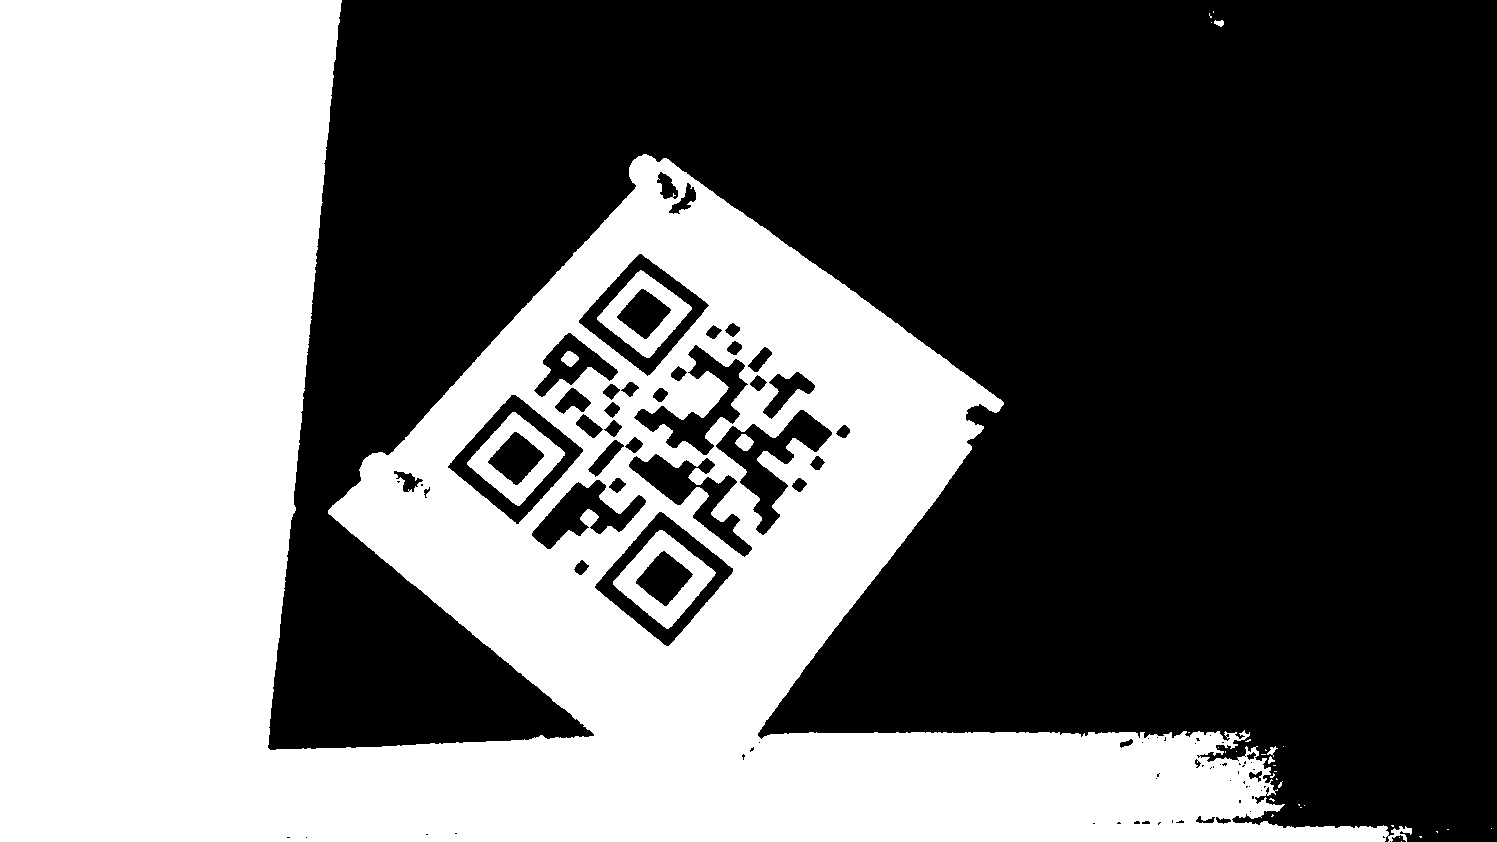
\includegraphics[scale=0.12]{images/qrcode-adler-wand_1___BINARIZED___.jpg}
\hspace{5px}
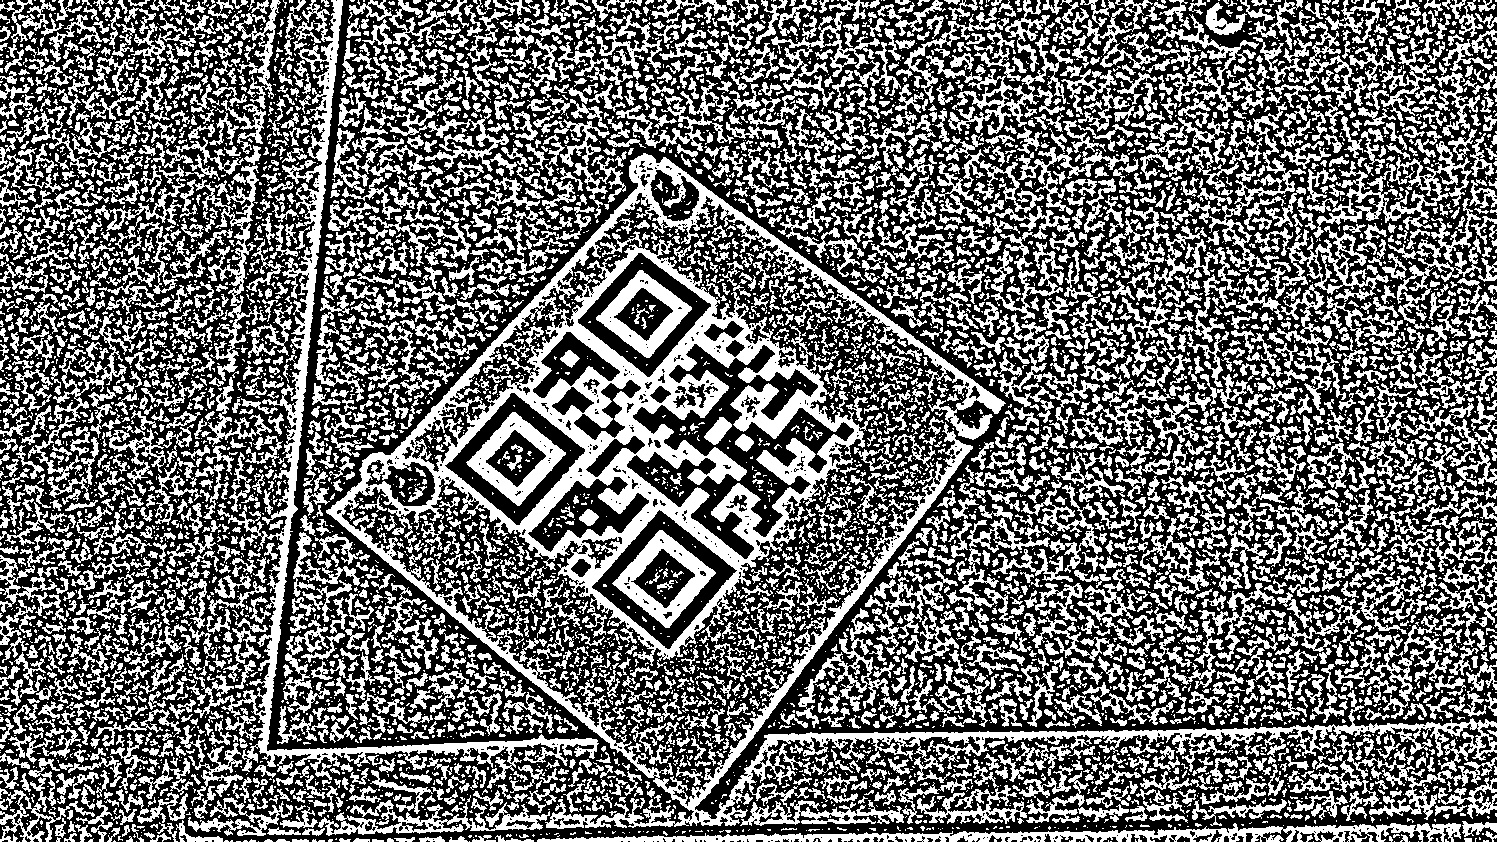
\includegraphics[scale=0.12]{images/qrcode-adler-wand_2___BINARIZED___.jpg}
\caption{Das Resultat der Binarisierung mit den jeweiligen Verfahren. Links global und Rechts lokal.}
\end{figure}

\textbf{Ausblick:} Durch das verändern des Parameters \texttt{C} in der \texttt{adaptiveThreshold} Methode kann eine ausgeglichenere Binarisierung erzielt werden. Diese Konstante wird von jedem Pixel abgezogen um einen Ausgleich zu schaffen. Allerdings können aus leicht Informationen verloren gehen!
